\chapter{Literature Review}%
\label{chapter:literatureReview}

\begin{introduction}
  Chapter II covers a review of the literature on vehicle maintenance and service quality at the dealerships. 
  Additionally, It analyses an existing system and compares it with the software solution of this dissertation.
\end{introduction} 


To acquire information about this topic I search information on the platform Scopus and Google Scholar. 
In Scopus, I used the query "Vehicle AND Maintenance AND dealerships" and found 49 papers.
On a primary analysis of the title and abstract, I selected 24 papers that were related to this topic.
However, on further examination, I chose to write about 3 papers in this dissertation. 
Most of the papers I discarded were because of the use of the words "Vehicle" and "dealerships". 
These words made the search return the papers that envisioned the dealerships as a reselling unit of the main company, which is not the focus of this dissertation.
Another reason was the use of machine learning to solve a specific problem, like predictive maintenance. 
While being a relevant approach, I decided to focus on Web Applications and vehicle maintenance concepts.

In Google Scholar, I found 3 papers about the electric vehicle in China. 
They may be important to understand the market in another country, however, I chose to not include them in this dissertation.  
The three papers I wrote in this dissertation were chosen because two of them were research studies about the process of vehicle maintenance and explained the importance of a quality of service in this industry.
The other paper described a solution implementation similar to the use case of this dissertation.

With these three papers, I could give a definition of the context and acquire some problems and solutions to focus on in the development phase.  

% \section{Background}

% The LightMobie is a company stablished in Águeda that provides a diverse set of products in the shared mobility sector. 
% The company also provides a software system to integrate with their bicycles and stations and vehicle maintenance.
% Currently, the company is in step of renewal of the system to a new solution of the bicycles and stations and is building a platform to interact and manage that system.
% This platform is able to visualize current and past information of the vehicle, stations and users and there interaction with each other.
% Additionally, alerts triggered by the equipment are also visible in the dashboard and the user can elaborate statistics on this data.


\section{Theoretical Concepts}

\subsection{Vehicle Maintenance}

Delivering vehicle maintenance services involves numerous activities, each crucial for maintaining service quality and ensuring customer satisfaction. 
Any deviation from these activities can negatively impact quality, leading to client dissatisfaction and loyalty loss. ~\cite{Setting_the_after_sale_process}
The loyalty of the client is the main source of income for the company, so it is important to maintain the quality of the service. ~\cite{Setting_the_after_sale_process}
To fulfill this requirement to the fullest, one must supervise every stage of the process. ~\cite{Setting_the_after_sale_process}


\begin{figure}[h]
  \caption{Macro-level Flow of a vehicle maintenance or repair service. This figure was inspired by figure 6: After Sales process from ~\citet{Setting_the_after_sale_process}.}
  \centering
  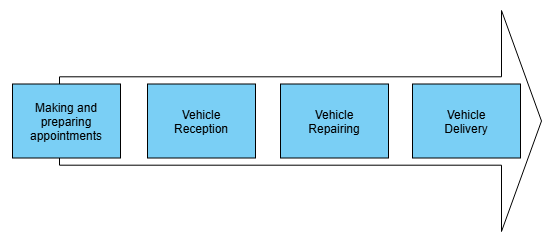
\includegraphics[width=0.50\textwidth]{figs/Vehicle_maintenace_macro}
  \label{fig:Vehicle_maintenace_macro}
\end{figure}

The general flow of vehicle maintenance is illustrated in the figure \ref{fig:Vehicle_maintenace_macro}. 
The first step of the process starts with a client interacting with the garage to schedule a vehicle maintenance or repair. 
After that, the client goes to the garage, where the receptionist receives the client and the vehicle.
Here, the mechanic will perform the maintenance of the vehicle and, when is done, the vehicle will be delivered to the client.

To ensure quality in the first step the receptionist must understand the fill capacity of the garage and the time to complete the job. 
With this information, the rececionist may accurately indicate the time to conclude the vehicle maintenance and get the client trust. ~\cite{Setting_the_after_sale_process}

In the second step, the receptionist and service advisor, when receiving the vehicle, must do a visual confirmation of the vehicle's condition. ~\cite{Setting_the_after_sale_process}
In this step, the receptionist explains to the client the services of the garage and they both agree with the services to be performed until a determined date. ~\cite{Setting_the_after_sale_process}

Following begins the third step and most important phase, the mechanic will perform the maintenance and repair of the vehicle. 
All of this process must be supervised by quality control to ensure that the job is done correctly. ~\cite{Setting_the_after_sale_process}
This includes the repair process, extra work, final tests, and service report. ~\cite{Setting_the_after_sale_process}
To accomplish that the use of a checklist is recommended to ensure precision and accuracy at each step. ~\cite{Setting_the_after_sale_process}

Finally, the last step is the delivery of the vehicle to the client. 
Here, the workshop manager must review the work done and the final price of the service to avoid extra payments from the client and incomplete payments to the workers. ~\cite{Setting_the_after_sale_process}

In this sense, the application of this dissertation will obey this flow.
For the receptionist and mechanic, the application will focus on reducing their mistake by giving accurate and illustrated information and making the work more effective.
And for the workshop manager to control the quality of the service with the assignment of tasks and authorization of purchases. 
Another user will be inserted into this flow, the warehouse operator, to manage the inventory of the dealership. 
The entire flow will be explained in Chapter III. 


\subsection{EMEL}
In june  i was able to visit the company \ac{emel}, that is a entity that operates and manage the bike sharing services of the public system of Gira.
This system operates 2.000 bicycles and 188 stations supporting a total of 12.000 to 14.000 trips per day.
With this number, the occurrence of equipment failure is much bigger so the efficiency in the process of maintenance is very apreciated.

The flow of a maintenance of a vehicle starts with there arrival at the workshop by a redistributor that discovers a malfunction during theres routine.
They fill a paper as see in \cite with the parts of the vehicle they find as faulted and do a simple search for vehicle eletric problems, namely if the gps is working and if the battery accepts charge.
If the vehicle fails this test it is put a side for a special worker to handle this problem, before the maintenance proceeds. Then, the vehicle goes to another waiting list waiting for a free mechanic. 
When chosen, the mechanic proceeds the mainteance fixing the problems identified in the paper and the others they find along the process.
After completing the maintenance, the mechanic fill the back of the paper with the parts he used to fix the vehicle, as seen in the figure \cite and the vehicle goes to another worker for its quality validation.
If the validation discovers a problem in the vehicle it returns to the mechanic that applied the maintenance to fix the problem, and then the vehicle waits for the redistributor to return it to the operacional ground.

The mainteannce provided by this company values more the efficiency than the quality due to the big workload it has. 
Since the evaluation is simple and superficial, more hidden problems may be overlooked and fail to address.

To manage the inventory at the workshop, the operators use an excel sheet to track the quantities of each part they have in stock. 
They periodically check the quantity available in stock for each part, so a system that informs the speed to which the parts are being use would be advantageous.
They have multiple supplier of vehicle parts, each with a determined quantity until a given date. 
They lack the tools to keep the contracts in check so to know when to realease another public tender for another supplier.

A system that address this issues would help the organization to manage their's inventory.


\subsection{Computerized Maintenance Management System}

The software solution i will develop is a \ac{CMMS}.
A \ac{CMMS} is able to centralize and automate the management of maintenance operations, helping the dealership to manage the work tasks and the inventory, providing metrics to optimize the maintenance process.

It maintains a database with the information about the equipment, maintenance schedules, work orders, inventory, and personnel. 
It also document and reports all maintenance actions to facilitate the adherence to the regulatory standards ensuring the quality of the service. 
And analyzes the maintenance costs, downtime, efficiency, and other metrics to improve performence, optimization and reduce cost to the dealership.

The key benefits of the \ac{CMMS} are the improvement of the Preventive Maintenance, since it's easier to analyse the vehicle life and schedule a maintenance before the equipment failures occur; reduce costs, as the life of the vehicle is prolonged and the critical maintenace being avoided, this sofware provides a long-term cost saving; efficiency enhancement, by allowing the workers to focus on completing task instead of paperwork; and Regulatory Compliance, by keeping track and documenting the maintenance activities to comply by the organization standards. 

In conclusion, \ac{CMMS} provides a structured, data-driven approach to maintenance that enhances efficiency, reduces costs, ensures compliance, and ultimately supports the operational reliability of critical equipment and infrastructure.





\subsection{Service Quality}
SERVQUAL is a service quality concept that provides a multidimensional approach for comparing consumers' perceptions of service quality against their expectations. 
It emphasizes five core dimensions ~\cite{SERVQUAL_OLD}:


\begin{itemize}
   \item Tangibles – Physical facilities, equipment, and appearance of personnel.
   \item Reliability – Ability to consistently deliver services as promised.
   \item Responsiveness – Willingness to assist the customer and proactivity.
   \item Assurance – Demonstrate courtesy and knowledge and inspire trust and confidence.
   \item Empathy – Caring and treating customers as individuals.
  \end{itemize}

\begin{figure}[h]
  \caption{The 7-point Likert scale where the respondent may answer the question from strongly disagree to strongly agree. ~\cite{master_servqual_model}}
  \centering
  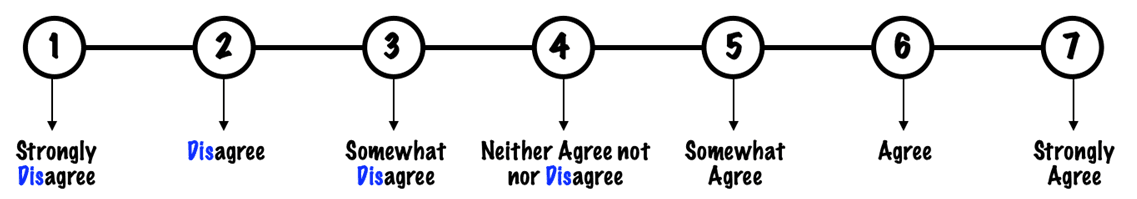
\includegraphics[width=\textwidth]{figs/likert_scale}
  \label{fig:likert_scale}
\end{figure}


To measure the quality of the service one needs to do a questionnaire composed of 22 questions that are divided into the five dimensions of the SERVQUAL model and are answer by the Likert's point scale, where the respondent may rate a question by strongly disagree to strongly agree, as seen in \ref{fig:likert_scale}. ~\cite{Measuring_After_sales_Service_Quality}
Each question must be divided into two answers, the first one is a score of the expectation of the service provided and the second one is the score of the perception of the service received. ~\cite{Measuring_After_sales_Service_Quality}
The difference between the two answers is the quality of the service. ~\cite{servqual_blog_da_qualidade} ~\cite{Measuring_After_sales_Service_Quality} ~\cite{SERVQUAL_OLD}

% In some cases is recommended to do two interviews with the same client, one before the service to aquire the expectations and another after the service to aquire the perception. ~\cite{servqual_blog_da_qualidade}
The authors of ~\citet{Measuring_After_sales_Service_Quality} used the SERVQUAL model to measure the quality of the service at a CMV SA dealership in South Africa.
They collected the data from a semi-structured questionnaire and interviews with customers, managers, and staff.
The questionnaire can be seen in the figure \ref{fig:SERVQUAL_statements}.

The results seen in figure \ref{fig:SERVQUAL_results} revealed a negative score in all five dimensions. 
Even comparing the expectations of the customers with the expectations of the dealers the average score was negative (-0.10).
This shows that the services provided by the CMV SA dealer are not meeting the expectations of the customers and further improvements are needed. ~\cite{Measuring_After_sales_Service_Quality}

The customer's recommendations included opening more workshops, to reduce travel inconvenience, and availability of parts, due to the long wait for the arrival from China.
The authors of ~\citet{Measuring_After_sales_Service_Quality} emphasize the importance of service quality to the success of the business and recommend that the dealer should conduct regular SERVQUAL assessments to monitor and address service quality gaps. ~\cite{Measuring_After_sales_Service_Quality}

To address this issue, I will develop in this dissertation another application for the clients. 
This application will allow the users to evaluate the service done in this dealership, as well as some recommendations, following the model SERVQUAL. 

% \section{Increase Clients Satisfaction in Vehicle Maintenance}
% In belgrade, serbia, in 2013, a research was conducted to measure the satisfaction of the clients at dealerships. ~\cite{Setting_the_after_sale_process}
% In the reasearch, they divided the consumers' expectations or demands in three categories:
% \begin{itemize}
%   \item quality of repair work, service done within the agreed time schedule, price, friendliness and professionalism, the time waiting for an appointment. 
%   \item availability of spare parts, advice given for further maintenance, information given about additional work. 
%   \item adequate documentation about accomplished work, replacing vehicles, to invoices explained, café, Wi-Fi, phone availability. In this paper only the first category has been taken into consideration. 
% \end{itemize}



% The GAP model, precedent from the SERVQUAL, also measures service quality by identifying the difference between customer expectations and actual perceptions. 
% These gaps include discrepancies between customer expectations and management's understanding, management's perceptions and service specifications, service specifications and actual delivery, actual delivery and communicated services, and expected and delivered service. ~\cite{Measuring_After_sales_Service_Quality}

% https://forms.app/en/blog/gap-model-of-service






\section{Existing solution}

\subsection{Fiix}
Fiix is a cloud-based \ac{CMMS} that allow organizations to manage their maintenance operations. 
It's main strengths lies on its advanced preventive maintenance scheduling, Comprehensive Work Order and Asset Management and AI-Powered Analytics and Reporting.

Despite the advantages of this software, Fiix has a high learning curve due to it's complexity and not intuitive old-fashion design interface. 
Also Fiix repordly lacks a built-in interal messaging system for crew communication. Most information sharing relies on notes and files attached to work orders, which may not be ideal for real-time collaboration.

With this effects in mind, i will aim in this software development to achieve a simple and user friendly solution where the users can intuitively interact with it by focusing on the key functional feature and easy navigation.

\subsection{Service Management for MAS Motors LLC}
MAS Motors LLC is a Toyota dealership that provides vehicle maintenance services in Libya.
This company handles the daily work manually using basic applications and paper documents.
This approach has proven to be ineffective with the expansion of the business and the company needs a more modern method. ~\cite{MAS_MOTORS}
So the author ~\citet{MAS_MOTORS} developed a web application that facilitates and increases the performance of the work at the dealership.

The system targets multiple user groups, such as service advisers, technicians, and customers, and offers a centralized platform to manage tasks like job card management, inventory updates, and customer service. ~\cite{MAS_MOTORS}
The authors' application was developed using Laravel, which is a PHP web application framework, with MariaDB as the database management system, which is a popular open-source relational database.

% The authors ~\citet{MAS_MOTORS} applied \ac{RAD} methodology as a software development tool to develop the application, due to its feedback, flexibility, and quickness.
% \ac{RAD} is an agile software development approach that focuses on rapid prototyping and quick feedback from users over costly planning. ~\cite{rapid_app_development}
% This approach ideology is an ongoing testing and refinement of the project instead of following a detailed planning and design, such as traditional models.

% It is composed of four phases: requirements definition, prototype, feedback, and final product. ~\cite{rapid_app_development}
% The requirement phase is defined by the definition of an unrestricted set of requirements, that can be changed during any point in the cycle. 

% In the prototype phase, the developers create a prototype of the system to Demonstrate to the client. 
% This prototype may be rushed since in the finalization stage, the developers will refine the final product. ~\cite{rapid_app_development}

% In the next phase, the feedback, developers present their work to the client and end-users.
% Depending on the feedback, the client may want to change the requirements or add something new. In this case, the developers will go back to the second stage and repeat the process. ~\cite{rapid_app_development}
% On positive feedback, the client is satisfied with the prototype and the developers will move to the final product phase.

% In the final phase, the developers will refine the prototype by optimizing their implementation. ~\cite{rapid_app_development}

% For the first phase, the authors write the requirements of the system following the Hewlett-Packard \ac{FURPS} model that categorizes the software requirements into functional and non-functional aspects.
% The acronym stands for:

% \begin{itemize}
%    \item Functionality – The core features and business-domain-specific aspects.
%    \item Usability – User interface considerations like accessibility and aesthetics.
%    \item Reliability – System availability, accuracy, and failure recovery.
%    \item Performance – Metrics such as response time and throughput.
%    \item Supportability – Testability, maintainability, and scalability.
%   \end{itemize}

The results of the application were positive, the survey response from employees and customers classified the system according to the \ac{FURPS} model with scores of 4.27 for functionality, 4.30 for usability, 4.27 for reliability, 4.46 for performance, and 3.36 for supportability.
Supportability was the lowest score, due to limited configuration options ~\cite{MAS_MOTORS}, however, the overall system improved the service efficiency and customer satisfaction. ~\cite{MAS_MOTORS}
The employees also recommended future enhancements, such as SMS notifications for service reminders, integrating social media, and expanding customer configuration options.

% This SMS notifications functionality will be planned in this dissertation Client application to inform the end of the maintenance and the availability for vehicle delivery. 
As noted by MARS Motors' Employees i will integrate an email notification service into the software, that is used on the lightmobie bike sharing system for alerts and user email validation and notification. 

\subsection{Architecture Comparison}

% The architecture of the application will have a \ac{MVC} pattern. 
% The \ac{MVC} pattern separates the application into three main components: Model, View, and Controller.~\cite{mvc_geeksforgeeks} ~\cite{MVC_StartupHouse}
% The Model is responsable for the storage of data and the logic of the application.  ~\cite{mvc_geeksforgeeks} ~\cite{MVC_StartupHouse}
% It provides an abstraction layer of the database that allows data operation without the direct contact from the user interface. ~\cite{MVC_StartupHouse}
% The View represents the \ac{UI} of the application and is used to present the information from the Model component. ~\cite{mvc_geeksforgeeks} ~\cite{MVC_StartupHouse}
% This component is also responsable for the user's interactions and it does not contain any logic of the application, only limits itself to the communication between the Controller and the user. ~\cite{MVC_StartupHouse}
% The Controller is responsable to process the data and update the Model and the view, based on the user's actions. ~\cite{mvc_geeksforgeeks} ~\cite{MVC_StartupHouse}

% This pattern provides a clean separation of concerns, that increases the maintainability, reusability and testability of the code. ~\cite{mvc_geeksforgeeks} ~\cite{MVC_StartupHouse}
% This requirements are advantageous, since the natural agility of the requirements of the project are not fully stablished and may receive some suggestion from the company along the way. 
% The scalability is also important since the aim market of this application are the company's dealerships that may be scattered across the country or even Europe.

The framework the application will be built with is the Asp Net Core MVC. 
I believe this approach will be better than following the successful application from \citet{MAS_MOTORS} due to a variety of reasons shown in \ref{table:architetcture_comparison}.

Firstly, the integration with the Microsoft framework MYSQL database is more simple when using ASP.NET Core due to the package Entity Framework. % [https://learn.microsoft.com/en-us/aspnet/entity-framework]
Laravel also supports this database interaction, but Asp Net Core MVC is more suitable for this environment. ~\cite{asp_net_vs_laravel}

Additionally, Laravel loses in performance with the compiled language ASP.NET since it is an interpreted language. 
Finally, in security, Laravel offers some security features like hashing or secure input validation but requires deeper PHP knowledge and proactive vulnerability management. 
Microsoft offers greater security tools in ASP.NET Core mvc with role-based authentication and login management with Identity framework.
These functionalities provide a major abstraction to this concept and allow the developer to focus on the application functionalities. ~\cite{asp_net_vs_laravel}


\begin{table}[]
    \begin{tabular}{| m{5em} | m{15em} | m{15em} |}
      \hline
   Parameter & Laravel  & ASP.NET Core MVC   \\
     \hline
   Language & PHP & C\#  \\
     \hline
   Performance & Lower Performance due to being an interpreted language & Higher performance due to being a Compiled language   \\
     \hline
   Security & Offers some Features like hashing and secure input validation & Provides major abstraction with Microsoft tools   \\
     \hline
   Integration with SQL & Supports various relational databases & More recommended for Microsoft environments because of integration packages  \\
     \hline
  \end{tabular}
    \caption{Comparison of the Laravel and ASP.NET Core MVC frameworks on a web application development to be integrated into LightMobie Platform.}
    \label{table:architetcture_comparison}
    \end{table}

  Another reason to use this framework is to integrate with the Fleet Management System that has the same approach. 
  This way, despite turning the system more complex, some functionalities like authentication and role assignment are already developed and only need integration. 
  This integration is not a disadvantage since I was involved in the construction of the system and I am familiar with the functionalities.
  
  

\section{Conclusion}

In this chapter i explained the theoretical concepts of the vehicle maintenance process in the literature and in the real case example EMEL in lisbon, and The SERVQUAL method to evaluate the quality of the service of a organization.
I also describe the existing solutions in the market, namely Fiix, and the results of MAS Motors LLC's application.
This solutions lack a intuitive interface and a notification service, so in this dissertation i will focus on accomplish that.

